% !TeX spellcheck = en_US
\chapter{State of the art}
\label{ch:stateoftheart}
\def\figdir{chapters/ch02_stateoftheart/figures}
	
%\begin{quote} 
%	\begin{flushright}
%		\textit{The greatest enemy of knowledge is not ignorance,\\ it is the illusion of knowledge.}
%		
%		--- ~ \textsc{Prof. Stephen Hawking}
%	\end{flushright}
%\end{quote}

%\paragraph*{State of art guidelines:}

%\begin{itemize}
%	\item \hl{Guide to the research p§lem (provide context, background).}
%	\item \hl{Show different approaches to a solution.}
%	\item \hl{Show the relevance to research problem, and need for further study.}
%\end{itemize}

\lettrine[lines=3,nindent=0em,loversize=0.1]{I}{n} this chapter, the role of urban vegetation in the urban climate is discussed. First, a general background of urban climate is given, with an introduction of the urban microclimate and its energy budget. The concept of urban heat island (UHI) and its implication on human comfort is provided after that. An overview of the relevant research on the impact of vegetation i1n urban microclimate is given including experimental and numerical methods. Based on the overview, the relevance of the research is indicated with specific research goals.

%, clearly indicating the underlying assumptions and limitations of the experimental and numerical approaches. 

\section{An overview of urban climate}

%However, as 30\% of the global population will be residing in cities, cities should strive to be sustainable and mitigate the present and future adverse effects on the climate. Furthermore, it is also in the interest of the city itself, as the city itself suffer from its unintended impacts. 

\begin{figure}[p]
	\centering
	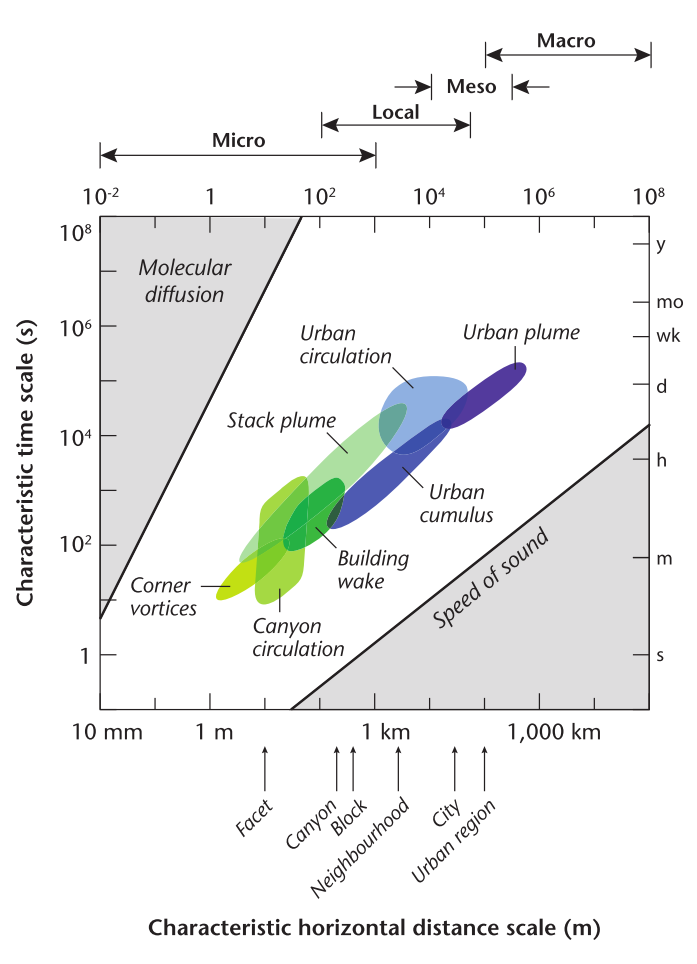
\includegraphics[width=0.7\textwidth]{\figdir/lengthtimescales.png}
	\caption{Time and length scale of phenomena in urban climate \citep{Oke2017a}.}
	\label{fig:lengthtimescales}
\end{figure}


``\textit{Urban climates are a prime example of inadvertent climate modification - the unintended impact of human activity on the atmosphere}'' \citep{Oke2017a}. In other words, the urban climate describes the modification of the atmosphere due to various components of the urban ecosystem. More specifically, the urban ecosystem modifies the natural environment through five aspects: atmosphere, biosphere, hydrosphere, pedo- and lithosphere, and the built system \citep{Oke2017a}. The urban atmosphere describes the influence of urban elements on the atmospheric conditions. The urban biosphere describes the influence of urban vegetation and other biological elements. The urban hydrosphere describes the water movement in the urban area, where the process such as surface run-off is described. The urban pedo- and lithosphere deals with the soil and ground modification in cities. Finally, the built system describes the influence of human-made structures on its environment. Therefore, the net urban climate is a result of these five aspects and the coupling between all these components is needed to be understood to study the urban climate.

%A study on the energy budget in an urban environment can provide a initial understanding of the coupling between varies processes in such an environment.



\subsection{Urban scales}

Due to the complexity of the urban area, in terms of its morphology and the associated climatological phenomena, the topology of the urban elements are typically simplified to various length scales. The urban elements are approximated at four length scales: micro (< km), local ($100$ m - $100$ km), meso ($10$ - $100$ km), and macro ($\num{e3}$-$\num{e5}$ km) scale. \cref{fig:lengthtimescales} shows the characteristic time and length scales in the urban climate \citep{Oke2017a}. The microscale resolves nearly all the topological features, resolving urban elements such as facets, individual buildings, and street-canyons. The local scale approximates the features of the microscale and only resolves topological variability between $100$ m and up to $100$ km such as an urban neighborhood. The local climate zone (LCZ) clustering scheme is used to approximate the microscale urban element features, parameterizing the topology using parameters such as building plan area density $\lambda_b$ (\%) (i.e., ratio of plan-view area of building to total surface area), canyon aspect ratio $\lambda_s$ (i.e., ratio of building height to building width) and mean roughness length $z_H$ (m). The mesoscale further approximates the urban topology, only resolving the features between $10$ km and $100$ km scales. Therefore, modeling the urban climate at microscale means resolving urban elements such as facet (i.e., roofs, walls) and buildings, and the climatic properties associated with them. At microscale, flow phenomena such as \textit{standing vortex}, \textit{corner vortices}, \textit{canyon circulation} and \textit{building wake} are typically present. We are interested in the influence of building morphology on the these flow phenomena along with the \textit{hygrothermal} and \textit{radiative} conditions (e.g. shadowing) around the buildings, as all these parameters have a direct influence on the \textit{pedestrian comfort}. Ergo, urban microclimate models are designed to describe these phenomena. In contrast, urban mesoscale  models which deal with length scales $\mathcal{O}(10)$ - $\mathcal{O}(10^2)$ km, are designed to capture phenomena of much larger time and length scales such as \textit{urban heat island}, \textit{urban plumes} and \textit{cloud and precipitation} \citep{Oke2017a}. In such models, microclimate phenomena are either neglected or parameterized to ensure their computational tractability.

\subsection{Urban boundary layer}

The atmospheric boundary layer (ABL) is modified over the city resulting in an urban boundary layer (UBL). The UBL during the day is divided into four distinct regions: urban canopy layer (UCL), roughness sublayer (RSL), inertial sublayer (ISL), and mixing layer (ML) \citep{Oke2017a}. Figure \ref{fig:ubl} shows the layout of these layers over a city. The UCL spans from the surface to the average building/tree height in cities. The RSL, consisting of the UCL spans from the ground up to 2-5 times the average height of buildings in cities. The urban microclimate phenomena cannot be neglected at this scale such as the geometry-dependent flow characteristics (i.e., vortices, flow circulation, and building/tree wake) and non-uniformity in the surface fluxes. In other words, the 3D nature of the cities becomes an essential factor in describing the flow and climate characteristics. Therefore, a study of urban climate in this domain requires the consideration of the spatial variability of the city. The ISL, typically between $25$ to $250$ m is above the RSL and the uppermost layer of the surface layer (SL). At this layer, the flow is only affected by the integral effects of the urban neighborhood, and the spatial variability is less than the RSL. Furthermore, the wind profile is well defined through logarithmic profiles. The ML is above the ISL spanning vertically from $250$ up to $2500$ m. During the day, due to heating of the urban surfaces, there is strong mixing present in this layer \citep{Oke2017a}. The ML is separated from the free atmosphere (FA) (i.e., where the surface influences are negligible) by an entrainment zone (EZ).

	\begin{figure}[t]
		\centering
		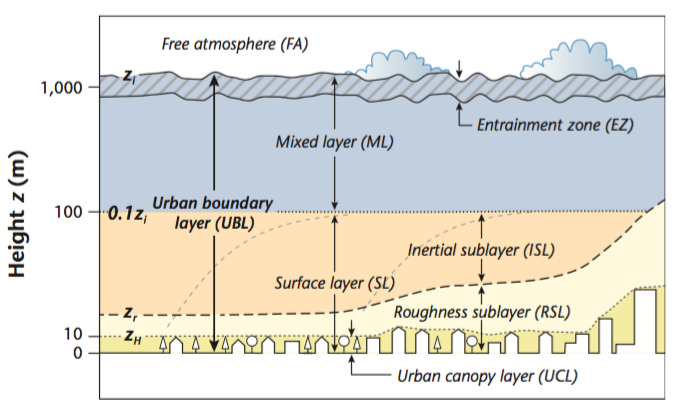
\includegraphics[width=\textwidth]{\figdir/ubl.png}
		\caption{Urban boundary layer during the day and divided into 4 distinct regions: urban canopy layer (UCL), roughness sublayer (RSL), inertial sublayer (ISL), and mixing layer (ML) \citep{Oke2017a}.}
		\label{fig:ubl}
	\end{figure}

\subsection{Energy balance}
\label{subsec:energybalance}

A study on the energy budget in an urban canopy layer can provide an initial understanding of the coupling between various processes in the urban microclimate. The energy budget can be determined by applying the conservation of energy for the UCL. The heat sinks and sources inside the domain are balanced by the fluxes at the boundaries. Figure \ref{fig:energybalance} shows a schematic representation of the energy balance applied to the UCL. 

	\begin{figure}[t]
		\centering
		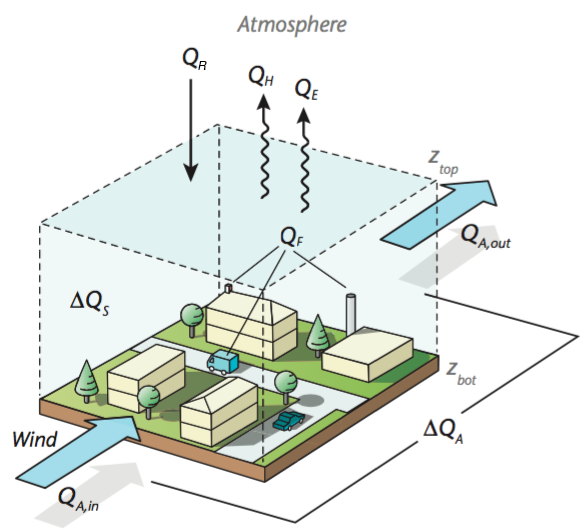
\includegraphics[width=0.7\textwidth]{\figdir/energybalance.png}
		\caption{The energy balance of an urban canopy layer (UCL) \citep{Oke2017a}.}
		\label{fig:energybalance}
	\end{figure}

The energy budget is defined as:
	\begin{equation}
	Q_r + Q_f = Q_s + Q_l + \Delta Q_t + \Delta Q_a
	\end{equation}
where $Q_r$ (W\,m$^{-2}$) is the net radiative heat flux, $Q_f$ (W\,m$^{-2}$) is the net anthropogenic heat flux, $Q_s$ (W\,m$^{-2}$) is the sensible heat flux, $Q_l$ (W\,m$^{-2}$) is latent heat flux, $\Delta Q_t$ (W\,m$^{-2}$) is the net energy storage change, and $\Delta Q_a$ (W\,m$^{-2}$) is the net energy advected by the wind into and out of the domain. In this thesis, the influence of vegetation on the energy balance in an urban microclimate is of focus. 

\subsection{Urban heat island}

Cities are known to experience higher temperatures than the surrounding rural areas \citep{Oke1973,Oke2017a}. The presence of unshaded, urban structures with low albedo and high thermal capacity, the lack of natural bodies such as open-water (e.g., ponds, rivers, and lakes), the lack of impervious surfaces (e.g., soil), and the lack of vegetation fraction is known to result in the UHI \citep{Bowler2010}. 
	
	\begin{figure}[t]
		\centering
		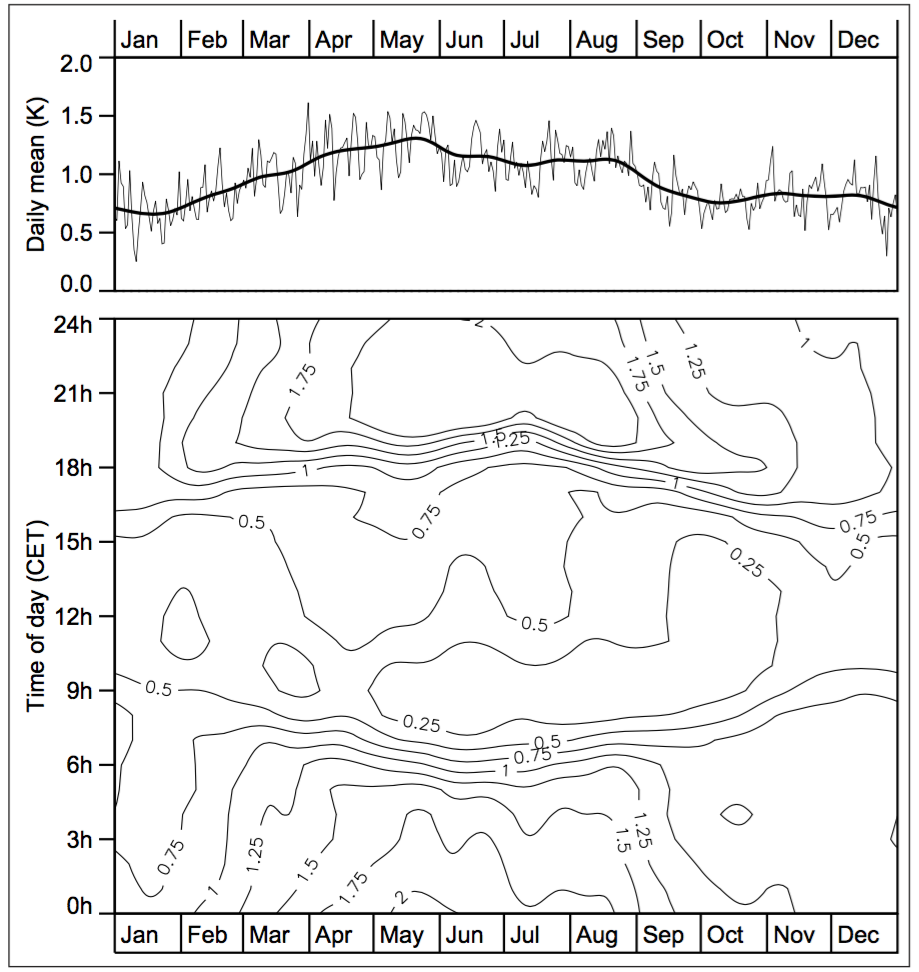
\includegraphics[width=0.7\textwidth]{\figdir/uhibasel.png}
		\caption{Daily and seasonal variation of UHI (K) in Basel, Switzerland \citep{Parlow2014}. The UHI is calculated as the air temperature difference between urban (Basel Spalenring) and rural area (Lange Erlen) obtained from hourly mean values for 1994-2003.}
		\label{fig:uhibasel}
	\end{figure}
The UHI-intensity is defined as the difference between the urban air temperature $T_{\textit{urban}}$ and the rural air temperature $T_{\textit{rural}}$. It provides a measure on warming associated to the presence of the city. \cref{fig:uhibasel} shows the daily and seasonal variation of UHI in Basel, Switzerland, where a UHI of up to $1.5$ $^{\circ}$C is observed during the summer. More specifically, the figure shows $UHI_{\textit{UCL}}$, i.e., the air temperature difference urban and rural area using a fixed station with temperature sensors at the  height of urban canopy layer. The UHI has been shown to have a negative influence on human health and comfort in cities \citep{santamouris2001energy,Kovats2008,Salmond2016}. For examples, increased heat strokes and infant mortality during the heat wave has been observed in the past, such as in August 2003 summer \citep{Fouillet2006}. In future, the UHI effect is expected to grow due to increasing urbanization, which will lead to a predicted urban population of 5 billion by 2030 and 66\% of the world’s population living in cities by 2050 \citep{Seto2012, UnitedNations2015}. Furthermore, the temperatures in urban areas are predicted to further increase due to the combined effect of climate change with a projected $2-4$ \si{\celsius} increase in global average surface temperature by 2100 \citep{pachauri2014climate}. Thus, the detrimental effects of UHI are not only expected to grow but also is expected to affect more of the global population. Therefore, one of the driving objectives in cities is to mitigate this growing UHI and make cities more resilient and sustainable. 

\subsection{Human comfort}

One of the key aspects of the urban microclimate study is its impact on the urban population \citep{Oke2017a,Saneinejad2013}. The response and the state of the human body to the urban microclimate can be quantified through human physiological modeling. The energy balance of a human consists of heat flux from the body core to skin and the heat flux between the skin surface and environment:
	\begin{equation}
	Q_m + Q_w + Q_s + Q_l + Q_t =  \Delta Q_s
	\end{equation}
where $Q_m$ (W\,m$^{-2}$) is the heat produced from metabolism, $Q_w$ (W\,m$^{-2}$) is muscular activity, $Q_s$ (W\,m$^{-2}$) is sensible heat flux, $Q_l$ (W\,m$^{-2}$) is latent heat flux, $Q_t$ (W\,m$^{-2}$) is heat produced from respiration, and $\Delta Q_s$ (W\,m$^{-2}$) is the rate of energy storage. Various comfort models have been developed to solve the energy balance. The Munich Energy-Balance Model for Individuals (MEMI) solves energy balance with a two-node system solving the heat flux from the skin to the body core and heat fluxes through clothing \citep{Hoppe1999}. 

	\begin{figure}[p]
		\centering
		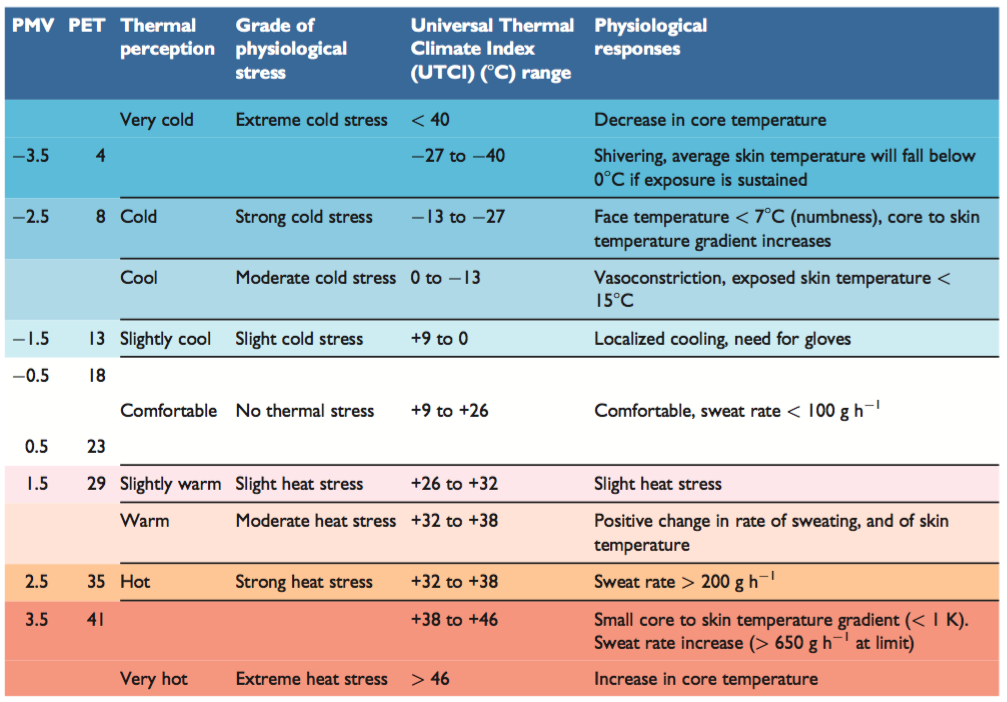
\includegraphics[width=\textwidth]{\figdir/thermalindex.png}
		\caption{Range, relation and physiological response for different parameters of the comfort indexes \citep{Oke2017a,Matzarakis1999,Bazejczyk2013}.}
		\label{fig:thermalindex}
	\end{figure}
	
	\begin{figure}[p]
	\centering
	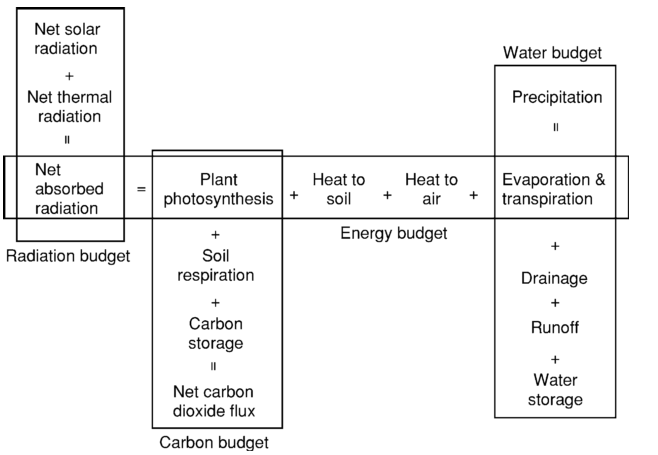
\includegraphics[width=\textwidth]{\figdir/energymassbudget.png}
	\caption{Coupling between radiative, energy and water budget \citep{Sawinski2011}.}
	\label{fig:energymassbudget}
	\end{figure}


A more realistic model is the UTCI-Fiala model that uses a 12 element (head, face, neck, shoulder, thorax, abdomen, upper and lower arm, hands, upper and lower legs, and feet), 187-node model \citep{Fiala2001,Brode2012,Blazejczyk2012,Jendritzky2012,Bazejczyk2013,Lokys2015}. The physiological response can then quantify using various thermal/human comfort indexes such as predicted mean vote (PMV), perceived temperature (PT), OUT-SET*, physiological equivalent temperature (PET), universal thermal climate index (UTCI). The UTCI ($^{\circ}$C) is determined as:
\begin{equation}
UTCI = T + f \left(T,{T_{\textit{mrt}}},\left| \mvec{u}  \right|,RH\right)
\label{eq:UTCIstate}
\end{equation}
where it is a function of air temperature $T$, the mean radiant temperature $T_{\textit{mrt}}$, wind speed $|\mvec{u}|$ and relative humidity $RH$ \citep{Fiala2001,Brode2012,Blazejczyk2012}. The mean radiant temperature $T_{\textit{mrt}}$ is influenced by the long-wave and the short-wave radiation, which is a function of direct solar radiation $q_{\textit{r,sw}}$ and the solar altitude $\phi$. The mean radiant temperature $T_{\textit{mrt}}$ ($^{\circ}$C) is defined as: 
\begin{equation}
T_{\textit{mrt}} = \left( T_{\textit{umrt}}^4  + \frac{f_p a_b}{\epsilon_p \sigma} q_{\textit{s,dir}} \right)^{\frac{1}{4}}
\label{eq:Tmrt}
\end{equation}
where $T_{\textit{umrt}}$ is the mean radiant temperature component belonging to the diffused or reflected part (i.e., from terrestrial source), $f_p$ is projected surface area of the person exposed to the sun, $\alpha_p$ is the albedo, $\epsilon_p$ is the emission coefficient and $q_{\textit{s,dir}}$ (W\,m$^{-2}$) is the direct solar radiation. The diffused/reflected component of the MRT is defined as:
\begin{equation}
T_{\textit{umrt}} = \left[ \frac{1}{\sigma} \sum_{i}^N \left(q_{\textit{r,i}} + \frac{a_b}{\epsilon_p} q_{\textit{s,i}} \right)F_i\right]^{\frac{1}{4}}
\label{eq:Tumrt}
\end{equation}
where $q_{\textit{r,i}}$ (W\,m$^{-2}$)  is the long-wave radiation emitted from surface $i$, $q_{\textit{s,i}}$ (W\,m$^{-2}$) is the reflected (assumed to be diffused) short-wave radiation from surface $i$, and $F_i$ is the view-factor between surface $i$ and the person. Figure \ref{fig:thermalindex} shows the various physiological responses at different values of various thermal indexes. The human body is defined to be in a comfortable state between $9\ge \mathrm{UTCI} \ge 26$ \si{\celsius}. Above this regime, heat stress occurs, where sweating rate and skin temperature starts to increase. The physiological stresses above comfort level are categorized as slight, moderate, strong and extreme heat stresses.

\section{Impact of vegetation on urban microclimate}

Urban greening solutions is seen as an effective tool to mitigate the growing UHI and improve the climate in urban areas \citep{Gillner2015, Bowler2010, Loughner2012}.  The energy contribution of the latent heat flux from vegetation in urban microclimate cannot be neglected as seen in section \ref{subsec:energybalance}. Furthermore, urban vegetation has a direct influence on the aerodynamic, radiative, thermal and moisture properties of the urban microclimate \citep{Oke1989}. Thus, the interaction of urban vegetation with the environment can be seen as the coupling between the radiative, heat and moisture balance, as depicted in \cref{fig:energymassbudget}. Therefore, to accurately assess the impact of urban vegetation on the urban microclimate, these coupled processes must be taken into account.
	
The influence of plants on the microclimate in an urban environment is of growing interest due to the need of mitigating detrimental effects of urbanization and climate change on urban air temperature \citep{Chen2006,Demuzere2014,Dimoudi2003,Matthews2017,Shashua-Bar2009b,Shashua-Bar2000a}. Plants modify the climate by intercepting solar radiation and by extracting heat from the environment through transpiration during photosynthesis \citep{nobel2009physicochemical}. Furthermore, the plant interferes with the airflow, extracting momentum and enhancing turbulent mixing \citep{Finnigan2009, Gromke2014, Sanz2003}. Due to the present growing need to ensure that cities are resilient and can mitigate the rising temperatures, proposed mitigation strategies are to be properly assessed and such assessment requires an adequate characterization of the effects of vegetation. 

Foliage density is known to have an impact on the wind sheltering provided by a plant \citep{Bitog2012b,Bitog2011b,Guan2003,Manickathan2018b}. The aerodynamic properties of vegetation can be expressed simply through porosity and drag coefficient \citep{Grant1998,Guan2003,Manickathan2018b}. The porosity and drag coefficient are known to depend on plant species \citep{Cao2012,Manickathan2018b,Rudnicki2004,Vollsinger2005}, age \citep{Dahle2010} and, for deciduous plants that shed leaves during winter, the parameters have been observed to vary seasonally as well \citep{Dellwik2019,Hwang2011,Maass1995}. It is known that plant porosity can have an impact on turbulent mixing \citep{Bai2012,Hiraoka2008,Manickathan2018b,McClure2017}, which is seen to directly impact the thermal and pollutant dispersion characteristics of air flow \citep{Conan2015,Gromke2008,Gromke2015c,Gromke2008a}. Plants with high foliage density are seen to have a detrimental effect on pollutant dispersion of below-canopy pollutant sources such as automobiles \citep{Nowak2006}. Nevertheless, a high foliage density is also shown to have a beneficial impact on the pedestrian thermal comfort due to increased shading provided by the plant \citep{Hwang2011,Morakinyo2017,Ng2012}. Foliage density is parameterized using the leaf area index (LAI) to describe the net area of leaves and leaf area density ($a$) to describe the foliage distribution within the plant volume. A dense plant canopy can result in a significant amount of solar radiation being absorbed resulting in a high leaf-to-air temperature \citep{Hiraoka2005,Leuzinger2007,Manickathan2018a}. Higher plant transpiration is then required to compensate for the high solar radiation absorption \citep{Manickathan2018b}, and this can result in a lower air temperature under the foliage \citep{Wong2003}. Studies have also revealed that plant transpiration rate varies not just due to atmospheric evaporative demand (AED) \citep{Kichah2012,Manickathan2018a,McVicar2012,Tuzet2003} but can also dynamically vary during the day with higher transpiration during morning than in the evening \citep{Huang2017,Tuzet2003}.

%These parameters are typically measured using optical techniques \citep{Cao2012,Grant1998,Guan2003,Liu2018,Manickathan2018b,Phattaralerphong2005} that may compromise on the spatial accuracy and destructive techniques such as defoliation of the plant \citep{Jonckheere2004,ONeal2002}. Solar radiation absorption within the foliage is known to depend primarily on the distribution of the leaf area density \citep{Kichah2012,Manickathan2018a,Park2018}.  
	
\subsection{Influence of vegetation on the energy balance}

The energy balance satisfies:
\begin{equation}
\underbrace{\mathrm{energy\ into\ leaves}}_{\mathrm{absorbed\ radiation}}
- \underbrace{\mathrm{energy\ out\ of\ leaves} }_{\substack{\mathrm{emitted\ infrared}\\\mathrm{heat\ convection}\\\mathrm{heat\ conduction}\\\mathrm{evapotranspiration}}} = \underbrace{\mathrm{energy\ stored}}_{\substack{\mathrm{metabolism}\\\mathrm{heat\ capacity}}}
\end{equation}
Typically, the energy storage is small with respect to heat gain and heat loss. The heat conducted and convected is the sensible heat and the heat loss due to evaporation and transpiration at the leaf surface is known as latent heat. The resulting formulation can be simplified to:
\begin{equation}
q_{\textit{rad,leaf}} + q_{\textit{sen,leaf}} + q_{\textit{lat,leaf}} = 0
\end{equation}
where $q_{\textit{rad,leaf}}$ is the net radiative flux (W\,m$^{-2}$) consisting of absorbed net radiation and the emitted radiation from the leaves. In the context of urban microclimate, the radiative heat flux is divided into two components: the short-wave radiative heat flux $q_{s}$ (W\,m$^{-2}$) and the long-wave radiative heat flux $q_{r}$ (W\,m$^{-2}$). The short-wave component is also known as the solar radiation as it describes the radiation emitted from the sun, dealing with the portion of electromagnetic spectrum consisting of UV, visible and near-Infrared (NIR) radiation. On the other hand, the long-wave component is known as thermal radiation as it describes the radiation emitted by terrestrial elements such as buildings, vegetation, and clouds. The portion of electromagnetic spectrum it occupies is above 2-5 $\mu$m. 

\begin{figure}[t]
	\centering
	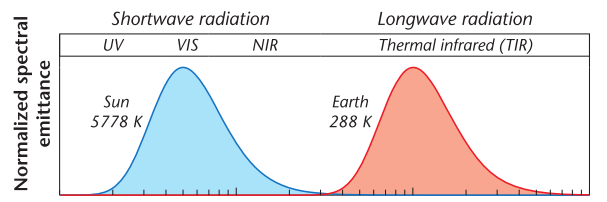
\includegraphics[width=0.9\textwidth]{\figdir/atmosphere_absorptionemission.png}
	\caption{Decomposition of the energy spectrum into two distinct parts: short-wave radiation $q_{s}$ and long-wave radiation $q_{r}$ \citep{Oke2017a}.}
	\label{fig:atmosphere_absorptionemission}
\end{figure}

Figure \ref{fig:atmosphere_absorptionemission} shows the spectral distribution associated to the short-wave and long-wave radiative heat fluxes, where it is simply a function of the temperature of the emitting body. The Stefan-Boltzmann law describes the radiative energy flux density $E$  (W\,m$^{-2}$) of a given body:
\begin{equation}
E = \varepsilon\,\sigma\,T^4
\end{equation}  
where $\varepsilon$ is the emissivity of body, $\sigma = \num{5.67e-8}$ W\,m$^{-2}$\,K$^{-4}$ is the Stefan-Boltzmann constant, and $T$ is the surface temperature (K). 

\begin{figure}[p]
	\centering
	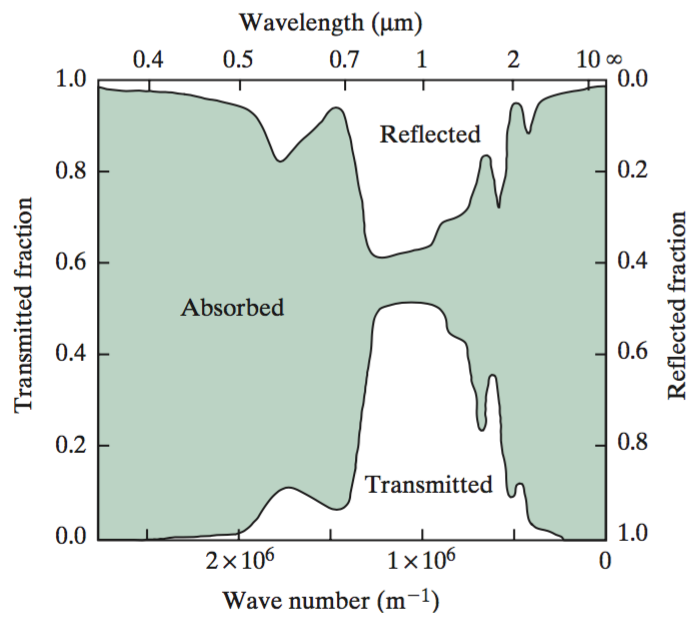
\includegraphics[width=0.7\textwidth]{\figdir/leaftransmission.png}
	\caption{Electromagnetic spectrum absorbed, transmitted, and reflected by a leaf \citep{Lambers2008,nobel2009physicochemical}. }
	\label{fig:leaftransmission}
\end{figure}

\begin{figure}[p]
	\centering
	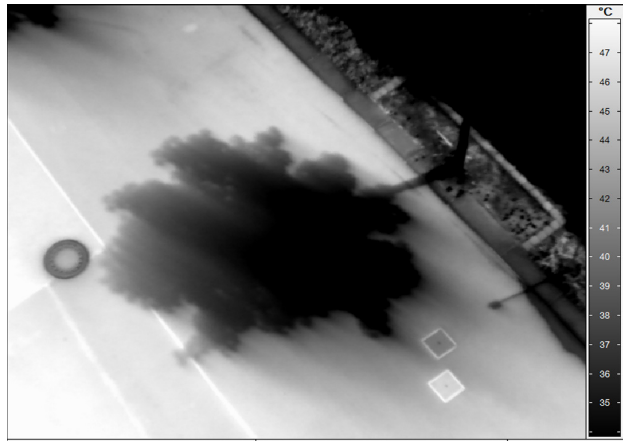
\includegraphics[width=0.7\textwidth]{\figdir/thermoimage.png}
	\caption{Infrared image assessing the shading effect of a tree (\textit{Tilia cordata}) on an asphalted streets \citep{Gillner2015}. }
	\label{fig:thermoimage}
\end{figure}	

Unlike buildings, which are regarded as opaque, vegetation is a semi-trans\-parent medium which transmits radiation depending on the wavelength. Figure \ref{fig:leaftransmission} shows the radiation absorption, transmission, and reflection fraction of a leaf. The leaves are semi-transparent to wavelength in between $0.5$ and $2$ $\mu$m. However, below and above these wavelengths, the leaves can be considered as an opaque medium absorbing all the radiation. Therefore, vegetation such as trees plays an essential role in the radiative balance in an urban area. Figure \ref{fig:thermoimage} shows an infrared image indicated the shading effect of a tree on an asphalt street, where a surface temperature drop of up to $15.2$ K was observable.

The sensible heat flux $q_{\textit{sen}}$ (W\,m$^{-2}$) is directly related to the temperature gradient:
\begin{equation}
q_{\textit{sen}} = h_{c,h} \left(T_{\textit{leaf}} - T_a\right)
\end{equation}
where $h_{c,h}$ is the convective heat transfer coefficient (CHTC) (W\,m$^{-2}$\,K$^{-1}$), $T_{\textit{leaf}}$ (K) is the leaf temperature, and $T_a$ (K) is the air temperature. Therefore, a larger temperature gradient or a larger CHTC results in larger sensible heat flux. Figure \ref{fig:leaftemperature_range} shows a typical range of leaf and air temperature during day and night. The leaf temperature is dependent on the photosynthetic rate and can either add or extract sensible heat from air depending on the sign of the temperature gradient.

\begin{figure}[p]
	\centering
	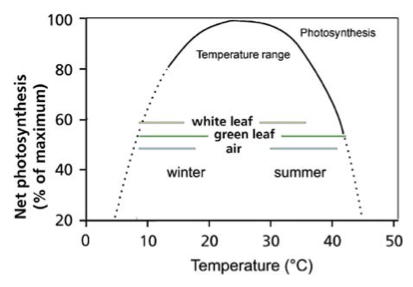
\includegraphics[width=0.5\textwidth]{\figdir/leaftemperature_range.png}
	\caption{Typical daily range of air and leaf temperature of glabrous green winter leaves and pubescent white summer leaves of \textit{Encelia farinosa} (brittlebush) \citep{Lambers2008}. }
	\label{fig:leaftemperature_range}
\end{figure}

\begin{figure}[p]
	\centering
	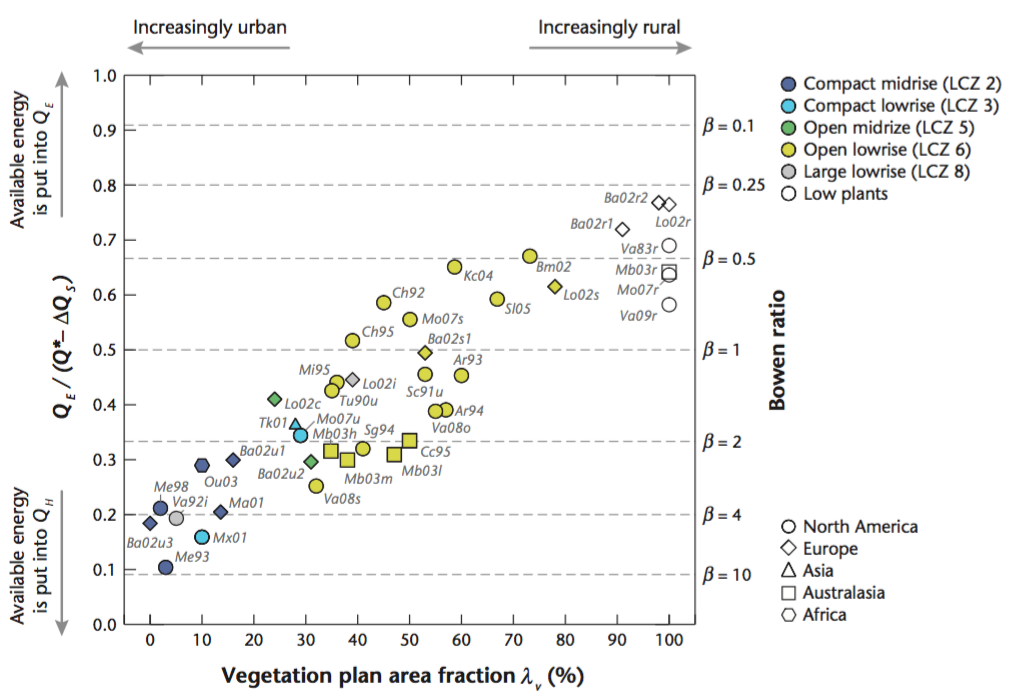
\includegraphics[width=\textwidth]{\figdir/vegetationfraction.png}
	\caption{Dependency of Bowen ratio $\beta$ to vegetation density for various cities around the world \citep{Oke2017a}. }
	\label{fig:vegetationfraction}
\end{figure}	

Finally, due to photosynthesis the latent heat flux generated from transpiration also has an impact on the energy balance. The latent heat flux $q_{\textit{lat}}$ (W\,m$^{-2}$) from the leaf surface is:
\begin{equation}
q_{\textit{lat}} = L_v g_{\textit{v,leaf}}
\end{equation}
where $L_v=\num{2.464e6}$ J\,kg$^{-1}$ (at $15$\si{\celsius}) is the latent heat of vaporization and $g_{\textit{v,leaf}}$ is the net evaporation and transpiration (i.e. evapotranspiration). During condensation, latent heat is released from water vapor in the air resulting in a temperature rise. During evapotranspiration, the opposite happens, where latent heat in the domain is increased, resulting in a temperature drop. Thus, the evapotranspiration rate of an urban area can become an effective strategy to extract the thermal energy from the environment. The resulting mitigation strategy is termed as evapotranspirative cooling \citep{Taha1997}. It has been observed that evapotranspirative cooling can generate oases that are up to $2-8$ \si{\celsius} cooler than other urban areas \citep{Oke1989,Taha1991}. An effective parameter that can give an insight into the cooling effect is the Bowen ratio $\beta$:
\begin{equation}
\beta = \frac{Q_s}{Q_l}
\end{equation}
where it is simply the ratio between sensible and latent heat fluxes. Cities with high Bowen ratio (such as $\beta > 1$) are attributed to having either lower vegetation density or litter open water surfaces and higher density of impervious urban structures. Figure \ref{fig:vegetationfraction} shows that there is a linear relationship between the Bowen ratio and vegetation density for various cities around the world. A higher vegetation density results in increased energy conversion to latent heat in the domain. However, it must be noted that the lower Bowen ratio can indicate higher humidity flux in the atmosphere due to increased evapotranspiration which can diminish the thermal comfort.

\subsection{Transpiration driven water cycle}

The water cycle driven by vegetation is a fundamental aspect of the influence of vegetation in cities. The transpiration driven or the vegetation water cycle is divided into three main aspects: water movement from soil to plant, water movement inside the plant, and finally the water movement from plant to the atmosphere. This process is the essence of the soil-plant-atmosphere continuum model, where the cohesion-tension theory is the mechanism used to describe the water movement \citep{Dixon1895}. 

An important variable used to define the state of water in various domains (e.g., soil, plant, air) is the water potential $\psi$. Water travels from high water potential to low water potential, and so, the transport of water can be determined merely from the water potential gradient. It is formulated as follows:
\begin{equation}
\mvec{g} = k\,\nabla \psi
\end{equation}
where $\mvec{g}$ is the water flux, $k$ is the conductance, and $\psi$ is the water potential. Therefore, for water to be supplied at the leaf from roots for transpiration, a sufficient gradient is required between the soil water potential and the leaf water potential. As the water demand at the leaves increases, a larger gradient will be required. Following this logic, water stress (i.e., difference between leaf water potential and soil water potential) is minimal before dawn and maximum during midday. 

\begin{figure}[t]
	\centering
	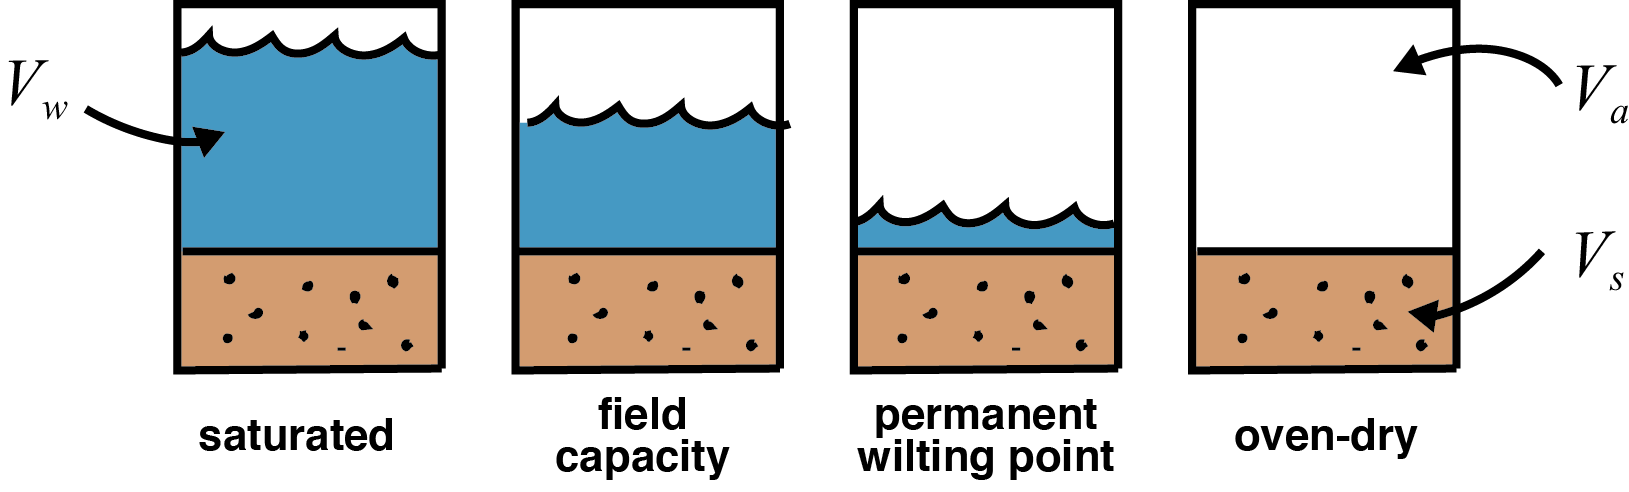
\includegraphics[width=0.7\textwidth]{\figdir/soilmoisture.png}
	\caption{Various degrees of soil moisture: $V_w$ is volume of water, $V_a$ is volume of air and $V_s$ is volume of soil.}
	\label{fig:soilmoisture}
\end{figure}

The water stress is magnified as the soil dries. Figure \ref{fig:soilmoisture} shows the various degrees of soil moisture that can exist. The volumetric water (or moisture) content $\theta$ (\%) is defined as the ratio of mass of water $V_w$ to the total volume $V$ (i.e. $V=V_w+V_a+V_s$),
\begin{equation}
\theta = \frac{V_w}{V}
\end{equation}
and provides a relative measure of volume of water. Similarly, the soil moisture content $w$ (kg\,m$^{-3}$) is defined as the ratio of mass of water $m_w$ to the total volume $V$
\begin{equation}
\theta = \frac{m_w}{V}
\end{equation}

\begin{figure}[t]
	\centering
	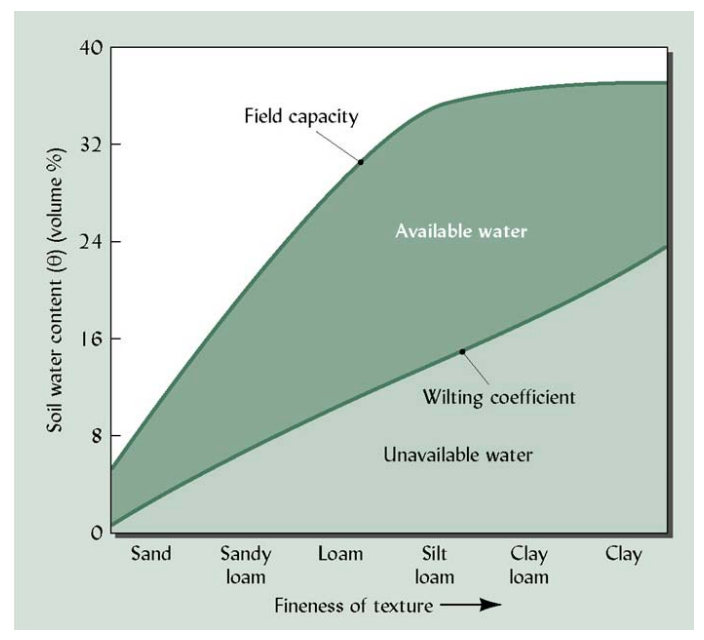
\includegraphics[width=0.7\textwidth]{\figdir/soilwatercontent.png}
	\caption{Soil water content for various soil types: sand, sandy loam, loam, silty loam, clay loam, and clay \citep{nobel2009physicochemical}. }
	\label{fig:soilwatercontent}
\end{figure}

The water content in the soil is maximum at saturated conditions, and as the soil dries, the soil moisture reaches the field capacity. The field capacity is the equilibrium state after an excess amount of water has drained away. As the soil dries further, the soil moisture reaches the permanent wilting point (PWP) or wilting point. Below the wilting point, plants start to wilt (i.e., the plant cells loose turgidity) and can no longer recover from the water stress. Typically, the wilting point is defined to be at a water potential of $\psi=-1.5$ \si{\MPa}. However, the water content associated with this water potential depends on the soil type. Figure \ref{fig:soilwatercontent} shows the regimes of field capacity and wilting point for various soil types. 
	
%	\begin{figure}[p]
%		\centering
%		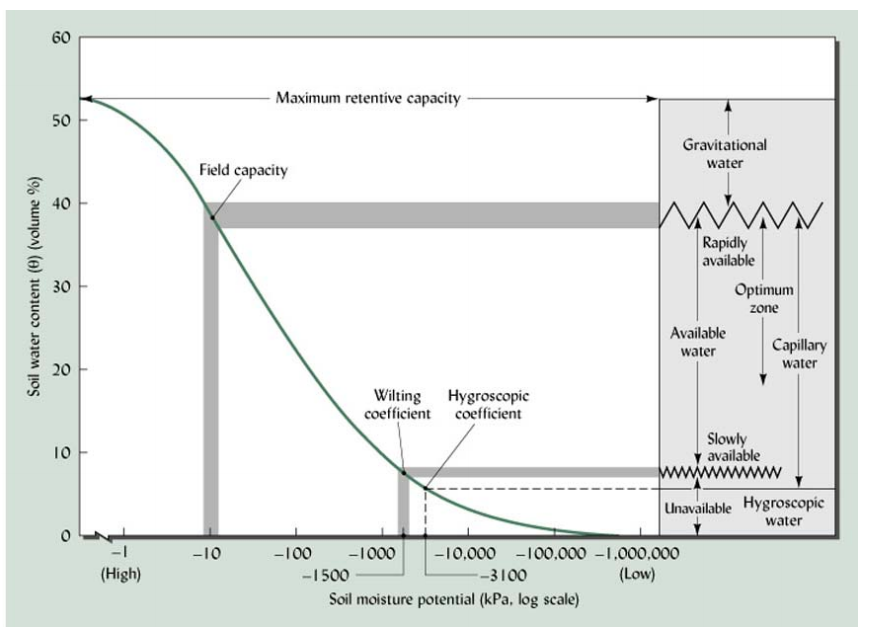
\includegraphics[width=0.7\textwidth]{\figdir/soilwatercontent_soilpotential.png}
%		\caption{A typical relation of soil water potential $\psi$ as a function of soil water content $\theta$ \citep{nobel2009physicochemical}.}
%		\label{fig:soilwatercontent_soilpotential}
%	\end{figure}

\begin{sidewaysfigure}[p]
		\centering
		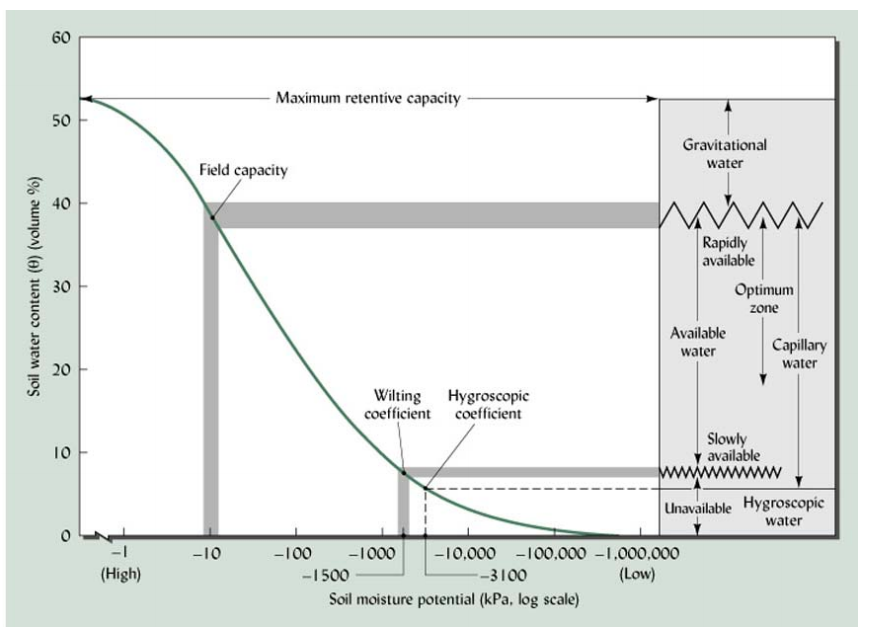
\includegraphics[width=0.9\textwidth]{\figdir/soilwatercontent_soilpotential.png}
		\caption{A typical relation of soil water potential $\psi$ as a function of soil water content $\theta$ \citep{nobel2009physicochemical}.}
		\label{fig:soilwatercontent_soilpotential}
	\end{sidewaysfigure}
	
	\begin{figure}[p]
		\centering
		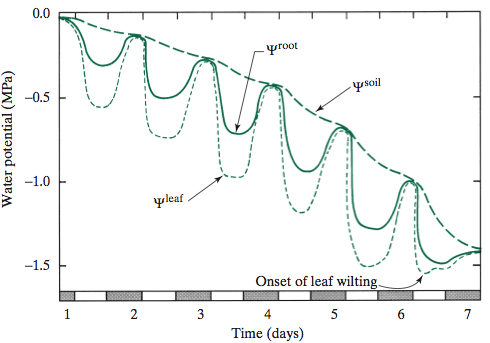
\includegraphics[width=0.7\textwidth]{\figdir/waterpotential_diurnal.png}
		\caption{Schematic representation  of diurnal change in soil, root, and leaf water potential \citep{nobel2009physicochemical}.}
		\label{fig:waterpotential_diurnal}
	\end{figure}	
	
A larger difference between field capacity and the wilting point indicates a larger availability of water for the plants. We see that sand cannot hold much water and furthermore, it quickly dries towards the wilting point. Whereas, loam and silt loam is seen to have a larger field capacity and buffer of water until it reaches the wilting point. Figure \ref{fig:soilwatercontent_soilpotential} shows the typical dependency of the soil water potential $\psi$ to the volumetric soil water content $\theta$ (i.e., ). The optimal zone for a plant is between the field capacity and around 10 orders of magnitude above the wilting point. The figure also shows that with high water content, water potential varies less. However, approaching the wilting point, the water potential drops exponentially, indicating a non-linearity in the water stress. 

Figure \ref{fig:waterpotential_diurnal} shows the diurnal response of soil, root and leaf water potential. We see that once the water potential too low, the onset of leaf wilting can compromise the transpiration driven water cycle and potential the health of the plant. Therefore, plants are more susceptible to lower soil moisture content, and in cities, water availability will become a critical factor, especially during a heat wave, for the survivability of the urban vegetation. 

%
%
%\begin{figure}[h]
%	\centering
%	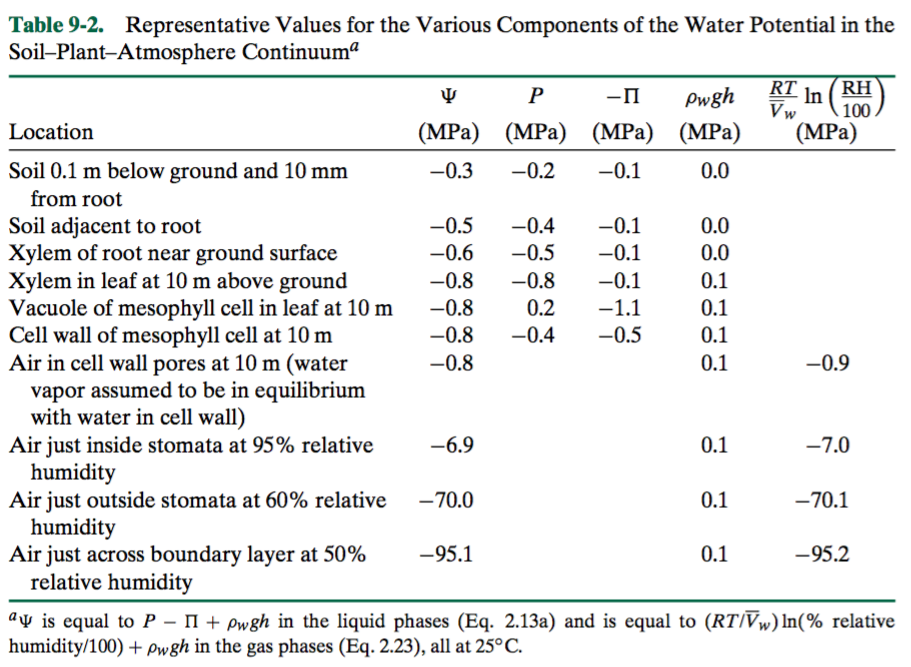
\includegraphics[width=0.7\textwidth]{\figdir/waterpotential_stdvalues.png}
%	\caption{waterpotential stdvalues}
%	\label{fig:waterpotential_stdvalues}
%\end{figure}
%


\section{Assessing impact of vegetation using experimental methods}

Various experimental approaches have been employed to assess the response of plants to environmental conditions ranging from field measurements \citep{Dellwik2019,Grant1998,Hagishima2007,Koizumi2016,Shashua-Bar2009b,Shashua-Bar2000a,Yuan2017}, greenhouse studies \citep{Fatnassi2006,Ganguly2009,Majdoubi2009,Montero2001}, and wind tunnel experiments \citep{Grace1977,Liu2018,Manickathan2018b,Miri2019,Rudnicki2004,Vollsinger2005,Yue2008}. Wind tunnel experiments, which provide the most control over the airflow conditions, typically focus on the aerodynamic characteristics such as drag coefficient, porosity, and sheltering effect of plants and neglect the hygrothermal responses of the plant \citep{Grace1977,Manickathan2018b}. Therefore, the relationship between porosity heterogeneity and hygrothermal conditions of plants has yet not been experimentally observed and characterized. Moreover, few studies provide a high-resolution temporal and spatial study of the hygrothermal conditions of the plant which can be used for validating numerical models. Thus, there is a need for high-resolution experimental datasets investigating the links between plant morphology, and atmospheric conditions including diurnal variations of the hygrothermal conditions such as air temperature, and relative humidity and how all of these affect plant conditions. 

\subsection{Field measurements}
Field measurements or ``\textit{in-situ}'' measurements provide the most realistic kind of measurements. There exist various measurement techniques for determining the evaporation or evapotranspiration. A summary of these techniques is provided below:

\begin{itemize}
	\item \textit{Pan evaporation}: Evaporation rate measured by measuring the change in volume of water in an open pan \citep{Finnigan1979, crowell2000guidelines, Farquhar2007, abtew2012evaporation}. It is one of the simplest and common technique to measure the water evaporation. 
	\item \textit{Lysimeters}: Lysimeters are used to measure the net evaporation and transpiration from the plant and soil \citep{Abtew1996,abtew2012evaporation}. 
	\item \textit{Eddy correlation}: Measures the vertical wind speed and local humidity at high temporal resolution \citep{German2000, shuttleworth1993evaporation}. The covariance of these two variables quantifies the water vapor flux, where $u_z'$ is the vertical fluctuating velocity and $w'$ is the fluctuating moisture content of air.
		\begin{equation}
		G_v = \tavg{u_z'w'}
		\end{equation}
	\item \textit{Bowen ratio}: The Bowen ratio dependent on the change in air temperature and vapor pressure provide an estimate for the net evapotranspiration by satisfying the urban energy balance \citep{Chen2006,Thom1975,DosReis1998,abtew2012evaporation,Deardorff1978}.
		\begin{equation}
		\mathrm{B} = \frac{Q_s}{Q_l} = \gamma \frac{\Delta T}{\Delta p_v}  
		\end{equation}
	\item \textit{Lidar}: Lidar or Light Detection and Ranging method can be used to sample the 3-D profile of water vapor concentration over the surface \citep{abtew2012evaporation,Idso1977}. 
	\item \textit{Remote sensing}: Remote sensing methods such as from a satellite instrument can also provide an estimation of the evapotranspiration rate \citep{Kustas1990,Melesse2008,Melesse2009,abtew2012evaporation}. 
\end{itemize}


\begin{figure}[t]
	\centering
	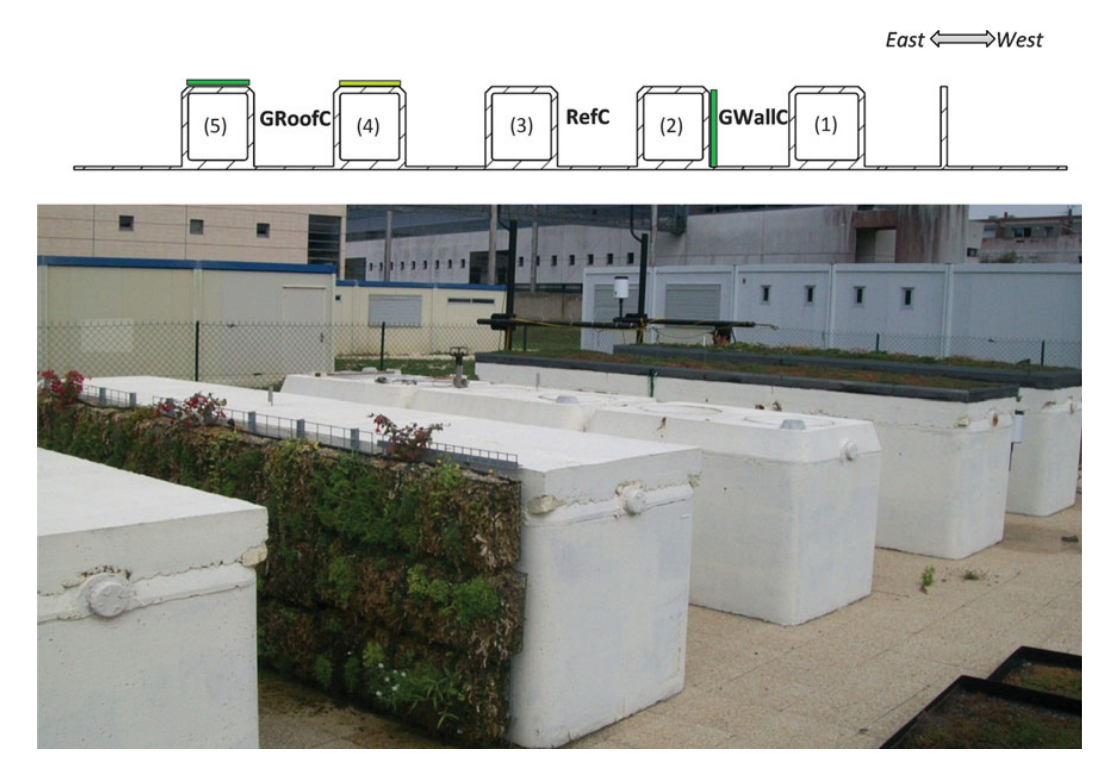
\includegraphics[width=\textwidth]{\figdir/hygrothermal.png}
	\caption{Microclimate study of green roofs and green walls in model street canyons \citep{Djedjig2015}}
	\label{fig:hygrothermal}
\end{figure}

However, a study on the mitigation potential of vegetation using such measurement is usually difficult as it requires a parametric study on the vegetation configuration. Authors have shown the possibility of hygrothermal measurements such as in a scaled street canyon to study the mitigation potential of vegetation such as green roofs or green walls \citep{Djedjig2015,Malys2014}. Figure \ref{fig:hygrothermal} shows a setup used to measure the microclimate of such green facades. Such reduced-scale studies enable to assess the impact of vegetation on the nearby building where configurations with and without vegetation can be assessed. Various authors have also studied the microclimate of crops in greenhouse \citep{Kichah2012,Baille1994,Roy, Montero2001,Fatnassi2006,Boulard2002}. Such studies provide a more controlled setup. The focus of such studies is to access the transpiration rate of plants and the microclimate developed around the plants and not necessarily towards the advancement of novel UHI mitigation strategies. 

\subsection{Wind tunnel measurements}

Similar to greenhouse studies, wind tunnel measurements provide a level of control that is seldom available from field measurements. Atmospheric boundary layer wind tunnel studies focus on trees in an urban setting \citep{Gromke2011,Gromke2008a}, measurements of flow past windbreaks \citep{Guan2003} or in forest canopies \citep{Bai2013,Conan2015,Kinnersley1994}, but are limited to the use of small model trees to match the size of building models typically used in these wind tunnel studies. This requirement prohibits the use of a larger mature natural tree. However, it is not known sufficiently to which extent small model trees can substitute such natural trees and whether both types display similar aerodynamic characteristics. There are several difficulties associated to scaling down of large natural trees to smaller model trees. Natural trees vibrate, deform and reconfigure, which all directly influence the drag and the resulting flow field around the tree \citep{Schouveiler2006,Tadrist2014,Vogel1989}. The mechanical properties of the tree are known not to scale linearly with size, so this fact should be considered when employing model trees to represent their larger counterparts \citep{DeLangre2008}. Moreover, predicting the dynamic response of a natural tree itself is a complex task due to the anisotropy in the material properties of the plant \citep{James2017}. The tree trunk wood of natural trees are known to have a radial anisotropy, resulting in a more complex mechanical response compared to isotropic materials \citep{Albrecht2016}. Furthermore, the location of the plant during its growth, for example forest-grown trees versus isolated trees, is known to alter the final form of the canopy architecture (James et al., 2014). Therefore, the plant growth history also plays a vital role in the plant morphology, and will result in a different mechanical response. Moreover, the age of the plant, varying from juvenile sapling to a mature plant, will further influence the mechanical properties of the plant. In this context, various authors have shown that the elastic modulus varies not only with species but also with the maturity of the plant \citep{Dahle2010,Macdonald2002,Telewski1995,Watt2008,Woodrum2003}. It is challenging to capture such allometric and morphological variability of different plants with small model trees. Without adequate care when designing the model trees, the response of model trees will not accurately represent natural trees that are found in an urban environment.

Furthermore, measurement techniques such as Particle Image Velocimetry provide a level of detail of the flow structure that is not possible from field measurements. The downside to wind tunnel measurements is the requirement for scale similarity and requirement for measurement facility. Various authors have successfully studied the flow characteristics of natural vegetation. \cite{Cao2012} compare various shrubby trees including a deciduous, coniferous, and broadleaf evergreen tree. The study investigated the dependency of drag and the overturning moment of various tree species to wind speed. Similarly, wind tunnel measurements are performed for hardwood species \citep{Vollsinger2005} and conifers \citep{Vollsinger2005, Mayhead1973, Bitog2011b}. These controlled experiments provide a better understanding of the influence of tree morphology on the drag coefficient. These measurements can be then used to improve existing computational fluid dynamics (CFD) models and accurately assess their impact on the flow \citep{Bitog2011b}. The PIV measurements of the tree wake can provide additional means of quantifying the turbulence modification due to trees in the flow \citep{Lee2012, Lee2014565}. Furthermore, these studies show additional understanding of sheltering provided by trees. The drag measurement is a useful tool to quantify the sheltering factor of the porous tree \citep{Guan2003,Kinnersley1994,Gromke2008a}. \cref{tab:windtunneltreeslit} briefly summarizes previous studies of drag forces on model and natural trees in wind tunnels. The natural trees are categorized into two types: hardwood and coniferous species. In these studies, the drag measurements are performed under airflow varying between $4$ and $20$ m\,s$^{-1}$. The main limitation of wind tunnel measurements is the height of the wind tunnel, as it restricts the maximum size of the measured trees. Nevertheless, these controlled experiments provide an improved understanding of the influence of tree morphology on the drag coefficient. They can improve the computational fluid dynamics (CFD) modeling of vegetation and respective model calibration, and thereby enable a more accurate assessment of the impact of vegetation on the environment \citep{Bitog2011b,Bitog2012b}. Additionally, wind tunnels enable non-intrusive flow measurements of the tree wake using particle image velocimetry (PIV). Such PIV measurements of the wake allow quantifying the impact on turbulence and the degree of sheltering provided by trees \citep{Lee2012,Lee2014565}.

{
	\ctable[
	caption = {Summary of previous studies measuring the drag coefficient of model and natural trees in wind tunnel.},
	label   = {tab:windtunneltreeslit},
	pos = p,
	mincapwidth = \textwidth,
	sideways,
	]{llrrl}{Scientific names: $^a$\textit{Thuja occidentalis Smaragd}, $^{b}$\textit{Hibiscus syriacus}, $^{c}$\textit{Thuja plicatas},\\
		$^{d}$\textit{Tsuga heterophylla}, $^{e}$\textit{Pinus contorta}, $^{f}$\textit{Alnus rubra}, $^{g}$\textit{Populus tremuloides}
	}{
		
		\FL
		Tree type 				&	Species 		 & 		$H$ (m) 		& $U$ (m\,s$^{-1}$) & References
		\ML
		model					& 	wood-wool		 & $0.115$ & $5.5 - 13.5$ & \multirow{2}{*}{\cite{Gromke2008a}} \\
		model					& 	sisal-fibre		 & $0.115$ & $5.5 - 13.5$ & 	\\[7pt]
		coniferous				& 	emerald cedar$^a$	 & $0.98$~~	& $5 - 15$~~~ & \multirow{2}{*}{\cite{Cao2012}} \\
		hardwood				& 	rose of sharon$^b$   & $1.24$~~	& $5 - 15$~~~ &  \\[7pt]
		coniferous				& 	western redcedar$^c$ & $1.95$~~	& $4 - 20$~~~ & \multirow{3}{*}{\cite{Vollsinger2005}} \\
		coniferous				& 	western hemlock$^d$  & $1.95$~~	& $4 - 20$~~~ & \\
		coniferous				& 	lodgepole pine$^e$   & $1.95$~~	& $4 - 20$~~~ & \\[7pt]
		hardwood				& 	red adler$^f$   	 & $1.95$~~	& $4 - 20$~~~ & \multirow{2}{*}{\cite{Vollsinger2005}} \\
		hardwood				& 	trembling aspen$^g$	 & $1.95$~~	& $4 - 20$~~~ & 
		\LL}
}


	\begin{figure}[t]
		\centering
		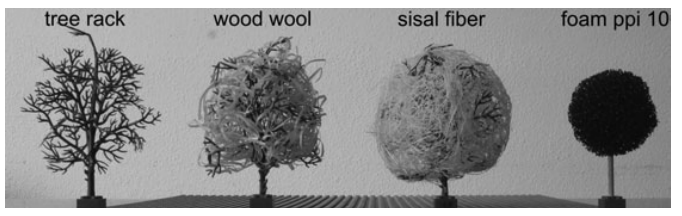
\includegraphics[width=\textwidth]{\figdir/modeltree.png}
		\caption{Different types of model trees used in wind tunnel studies \citep{Gromke2008a}. }
		\label{fig:modeltree}
	\end{figure}
	
	\begin{figure}[p]
		\centering
		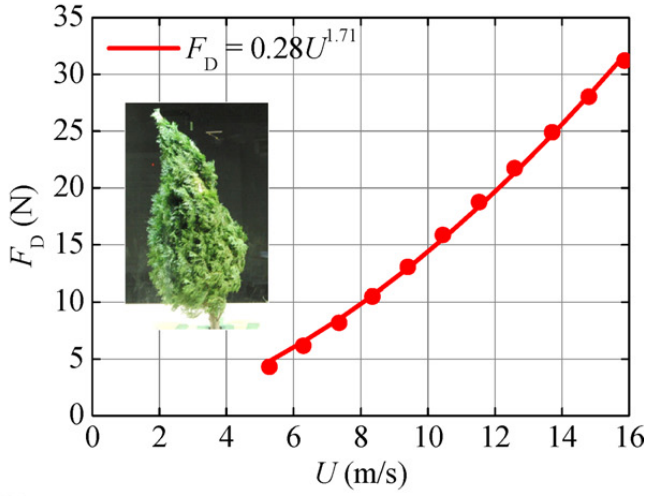
\includegraphics[width=0.7\textwidth]{\figdir/dragcoefficientree.png}
		\caption{Drag measurement study of small trees in windtunnel \citep{Cao2012}.}
		\label{fig:dragcoefficientree}
	\end{figure}
	
	\begin{figure}[p]
		\centering
		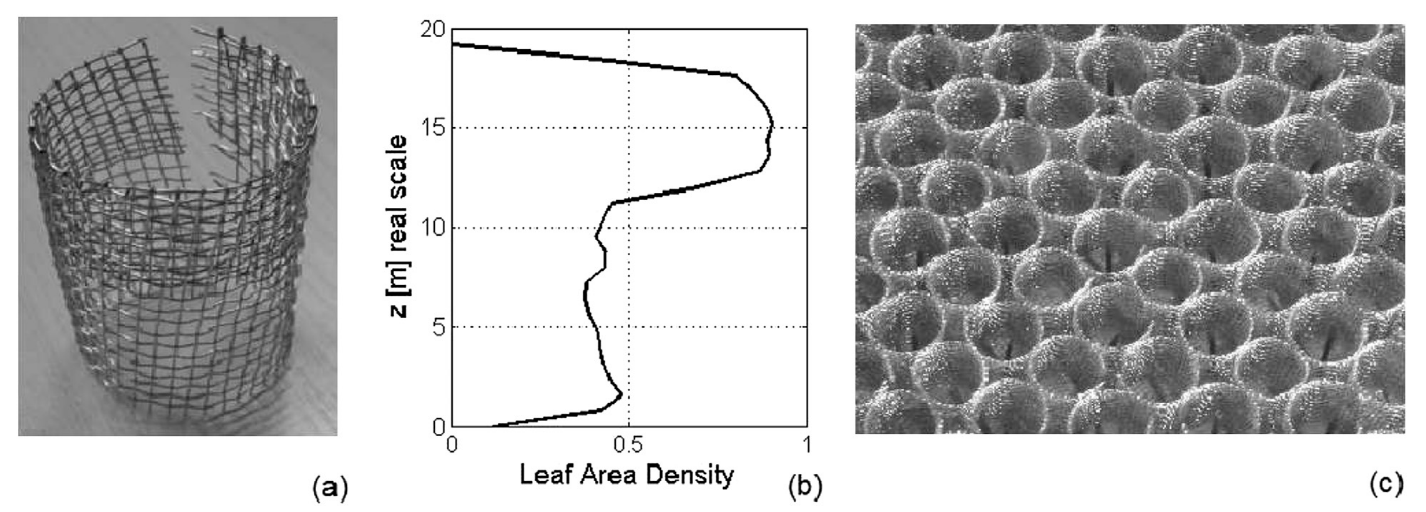
\includegraphics[width=\textwidth]{\figdir/modeltreecanoy.png}
		\caption{Wind tunnel model of a vegetation canopy from wire mesh  \citep{Conan2015}: \subfig{a} a picture of single mesh ring, \subfig{b} the vertical distribution of leaf area density $a$ of the single mesh ring and \subfig{c} an arrangement of multiple mesh rings to to model vegetation canopy flow.}
		\label{fig:modeltreecanoy}
	\end{figure}

Turbulent momentum exchange of vegetation with the environment was also investigated experimentally, such as in wind tunnels. In these studies, the flow field around the vegetation is typically correlated to its drag coefficient. \cite{Gromke2008a} investigated the flow around small model trees of various porosity and material, as shown in Figure \ref{fig:modeltree}. They used Laser Doppler Velocimetry (LDV) to perform a spectral analysis of the velocity, enabling to correlate the drag coefficient to the TKE dissipation. Investigations for natural, flexible trees were performed by \cite{Rudnicki2004} and \cite{Vollsinger2005}, where the effects of pruning and streamlining are quantified using drag coefficient measurements. \cite{Cao2012} employed a similar approach and investigated the impact of volumetric density on various deciduous, coniferous, and broadleaf evergreen trees (Figure \ref{fig:dragcoefficientree}). However, a detailed experimental study on the influence of natural vegetation on the flow using detailed flow field measurements nor a study of combining vegetation and a built environment is not available in the literature. The evolution of the turbulent flow field within the vegetation is difficult to measure in a wind tunnel using imaging techniques such as PIV as the flow inside is occluded by the foliage from the camera. However, the knowledge on the relation between turbulent production and dissipation within the vegetation is an essential determinant for the exchange processes of vegetation and the airflow. The simplest representation of trees is a porous fence. Various authors in the past have studies the flow past a thin porous fence: \citep{Gandemer1979, Dong2010, Perera1981,Hagen1971,Conan2015}. The model construction approach has also been extended to study flow past 3D dense vegetation and to study the flow through vegetation canopy \citep{Conan2015,Poggi2004}. Figure \ref{fig:modeltreecanoy} shows a typical construction of vegetation canopy for wind tunnel studies. Such studies enable to understand passive scalar transport modification such as pollution dispersion due to vegetation \citep{Gromke2011,Gromke2008}. A more advanced model constructions have also been employed where fractal type porous structures are made to mimic the tree structure \citep{McClure2017}. Authors have also modeled a resolved tree canopy using fractal dimensioning \citep{Bai2012,Bai2014a}. 

\section{Assessing impact of vegetation using numerical methods}

The global influence of vegetation on the local climate has been assessed by using urban microclimate models \citep{Bruse1998, Robitu2006}. There are two distinct classes of modeling the flow past vegetation: resolved approaches \citep{Endalew2009,Endalew2006} and unresolved approaches using porous media approaches \citep{Sanz2003, Kenjeres2013, Gromke2014, Katul2004}. In the resolved type of numerical methods, the elements of vegetation are directly resolved, where the Dirichlet and Neumann boundary conditions are directly prescribed. When employing a porous media approach, vegetation is simplified to representative volume elements, defined through the leaf area density $a$ ( or $\textit{LAD}$) (m$^2$\,m$^{-3}$):
\begin{equation}
a = \frac{A_{\textit{leaf}}}{V}
\end{equation}
defined as the ratio between one-side leaf surface area $A_{\textit{leaf}}$ in a given volume. 

%	\begin{figure}[h]
%		\centering
%		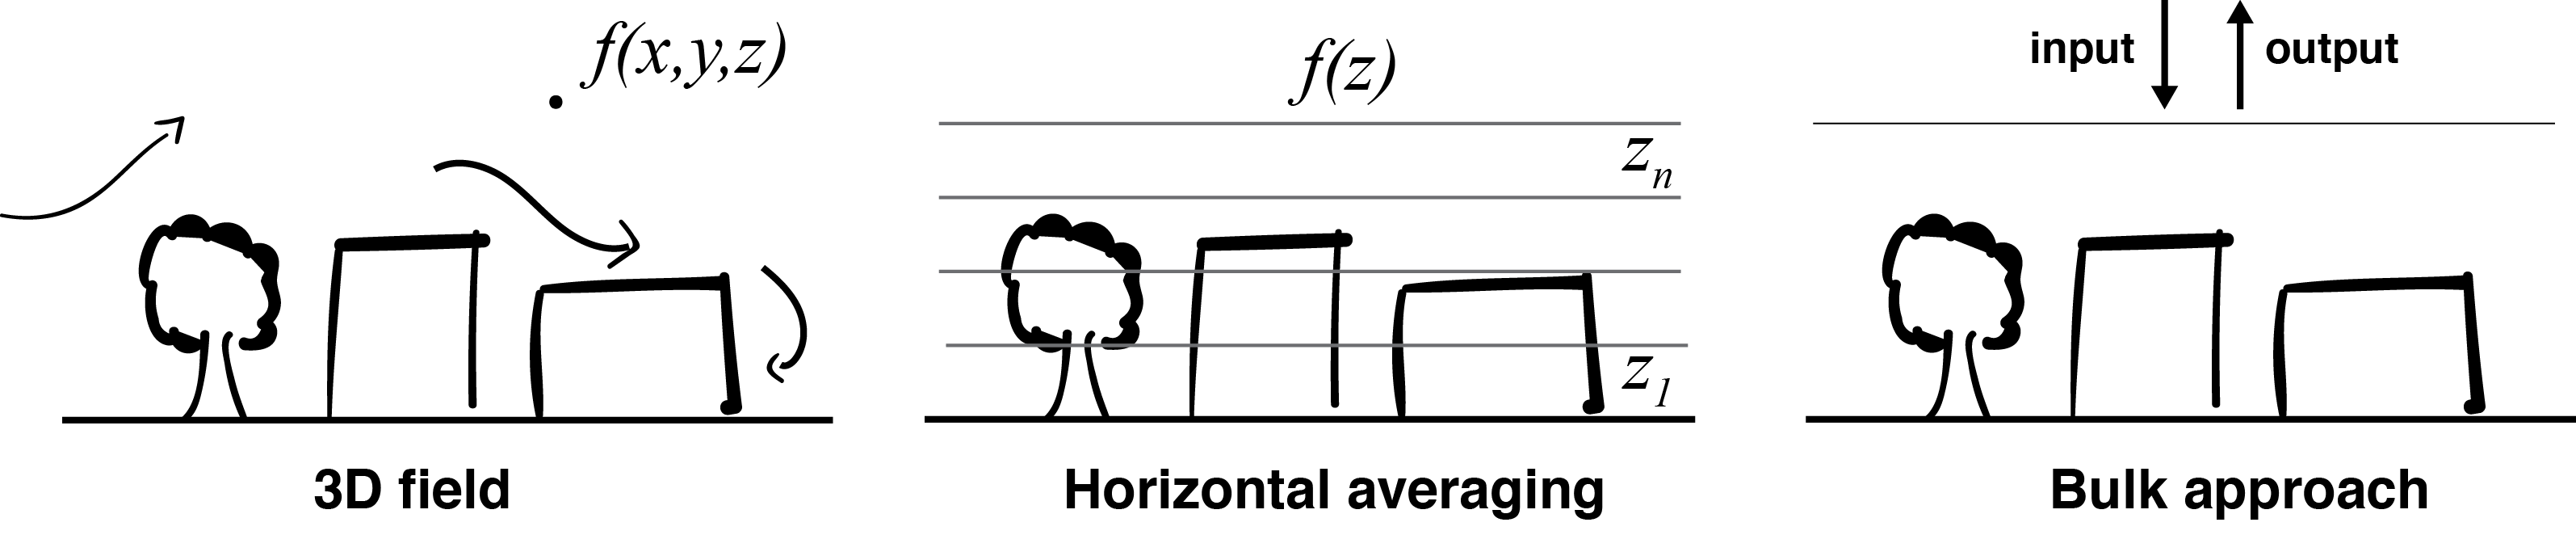
\includegraphics[width=0.99\textwidth]{\figdir/averagingapproaches.png}
%		\caption{Averaging approaches}
%		\label{fig:averagingapproaches}
%	\end{figure}	

\subsection{Integral energy budget models}

There exist various approaches to model evapotranspiration $E$ \citep{abtew2012evaporation}: 

\begin{itemize}
	\item \textit{Temperature-based methods}: The evapotranspiration is determined empirically from air temperature.
		\begin{equation}
		E = f(T)
		\end{equation}
	\item \textit{Radiation-based methods}: The evapotranspiration is determined from an empirical relation from downward short-wave radiation.
		\begin{equation}
			E = f(Q_{r,sw}) \qquad \mathrm{or} \qquad E = f(T,Q_{r,sw})
		\end{equation}
	\item \textit{Energy balance methods or Penman-Monteith method}: The evapotranspiration is determined from the urban energy balance, taking in account of the momentum transfer, mass transfer, heat storage, and heat conduction:
		\begin{equation}
			E = \frac{1}{\lambda} \frac{\Delta \left(Q_{r,net}-Q_c\right) + \rho c_p k_a \left(p_v - p_d\right)}{\Delta + \gamma \left(1 + \frac{k_a}{k_c}\right) }
		\end{equation}
	where $k_c$ is the canopy conductance.
\end{itemize}

In literature, several approaches have been used to model the heat and mass exchange of vegetation with the air. The big-leaf approach treats the whole canopy as a single leaf to determine the exchanges between vegetation and environment \citep{2861,Shuttleworth1985,Sellers1996}. A dual-big-leaf approach can differentiate sunlit and shaded leaves, providing an improvement to the big-leaf model \citep{Dai2004}. As an extension to these models, a multi-layer model segments the vegetation into layers, introducing a vertical heterogeneity concerning evapotranspiration in the vegetation \citep{Wang1990,Leuning1998}. These vertical energy budget models are used as simple representations of vegetation in urban microclimate models \citep{Dolman1993,Krayenhoff2014,Ryder2014}. 

\cite{HefnySalim2015} showed that numerical models should take into account the influence of trees without gross averaging approaches or surface parameterization and instead at least employ explicit approaches such as representing trees by porous media. This is especially important when wind flow patterns are the driving factors of the microclimate. Furthermore, parameters such as wind direction and foliage density and its interaction with urban configuration can be studied. Therefore, computational fluid dynamics models are seen as a better approach to achieve this goal. Such explicit methods allow to take into account parameters such as wind direction, and foliage density distribution. To represent trees as a porous medium, their drag coefficient is required and is typically assumed to be constant and independent of wind speed, and dependent only on tree species \citep{Wilson1977}. 

\subsection{Computational fluid dynamics model}

\subsubsection*{Turbulent momentum exchange}
%Fig. \ref{fig:wakezone} shows characteristics of the tree wake the that is aimed to be modeled using porous media approach. 
%
%\begin{figure}[t]
%	\centering
%	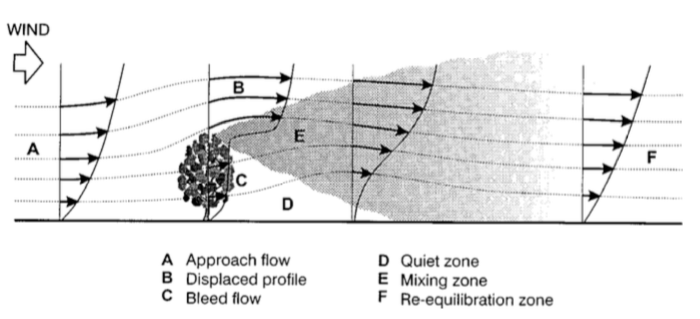
\includegraphics[width=\textwidth]{\figdir/wakezone.png}
%	\caption{Schematics of airflow regimes around the tree \citep{Cleugh1998,Judd1996}.}
%	\label{fig:wakezone}
%\end{figure}
%
%An arbitrary filtered field is defined as:
%
%\begin{equation}
%\phi = \eavg{\phi} + \phi''
%\end{equation}
%
%where $\phi$ is a given field,  $\phi$ is the dispersion field, and the filtered field is:
%\begin{equation}
%\eavg{\phi} = \frac{1}{V} \int \phi\ dV 
%\end{equation}
%Various authors study the flow past porous fences: $k-\varepsilon$ \citep{Packwood2000, Bourdin2008}. \cite{Cleugh1998} also investigate the influence of airflow on the microclimate.


To represent trees as a porous medium, their drag coefficient is required, which is typically assumed to be constant, independent of wind speed and tree species \citep{Wilson1977}. The porous media formulation of vegetation is obtained from the filtered Navier-Stokes where the filter is the representative volume element (REV). The filtered Navier-Stokes equations used for porous media formulation of vegetation has two additional terms:
\begin{equation}
-\frac{1}{\rho}\eavg{\nabla p''} + \nu \eavg{\nabla^2 \mvec{u}''}
\end{equation}
where the first term is the contribution due to pressure $p$ and the second term is the viscous contribution of the plant at velocity $u$. The problem is closed using Darcy-Forcheimer type force equation: 
\begin{equation}
F_{d} =  a_1 U^2 + a_2 U 
\end{equation}
and typically, the viscous drag is assumed to be negligible compared to the form drag \citep{Raupach1981, Sanz2003}. So, the effect of vegetation on momentum is described by the following expression:
\begin{equation}
\mvec{f} = c_d a \mvec{u}|\mvec{u}|
\end{equation}
where $a_1 = c_d\,a$, $c_d$ is the leaf drag coefficient (-) and $a$ is defined as leaf area density (m$^2$\,m$^{-3}$) defining a spatially varying vegetation density. During the simulation, the drag coefficient and leaf area density are usually fixed. However, \cite{DeLangre2012} shows that flexible tree foliage undergoes reconfiguration, particularly at high wind speeds as the leaves and branches reorient themselves along the wind direction. Such reconfiguration influences the flow through trees and the resulting drag coefficient. Similar findings are made during in-situ measurements of mature trees \citep{Grant1998,Kane2006,Koizumi2016}. Turbulent momentum exchange of vegetation with the environment employing Computational Fluid Dynamics (CFD) was initially investigated for canopy flow, mainly using the Reynolds-Averaged Navier Stokes approach (RANS). \cite{Wilson1977} developed a one-dimensional mathematical model for turbulent airflow around vegetation canopies with closure for mean momentum, turbulent kinetic energy (TKE) and turbulent dissipation rate (TDR).  \cite{Liu1996} determined source/sink terms for a two-dimensional $k-\varepsilon$ model, thereby modeling vegetation as a porous media. They investigated the eddy diffusivity past a forest edge and discussed the accuracy and limitation of employing the two equation closure model. \cite{Liang2006} improved the  $k-\varepsilon$ closure model for vegetation with additional terms and investigated 3D flow past a small forest immersed in atmospheric boundary layer flow. Regarding the urban environment, \cite{Kenjeres2013} assessed the turbulent flows in urban areas with vegetation using a $k-\varepsilon$ turbulence closure. \cite{Bruse1998}, \cite{Robitu2006} and \cite{Gromke2015c} also employed the  $k-\varepsilon$ turbulence closure or a modified  $k-\varepsilon$ model for urban studies. Such RANS approaches are usually employed to investigate the turbulent momentum exchanges between three-dimensional heterogeneous vegetation and the environment. Some authors have also employed large-eddy turbulence modeling approach (LES) for the canopy flows \citep{Maruyama2008, Lopes2013,Shaw1992,Moonen2013}. These approaches enable instantaneous realizations of the turbulent velocity and scalar fields. The benefit of such model is that the turbulence closure due to vegetation requires less empirical formulation  \citep{Hiraoka2011,Lopes2013}.  However, the downside is the high computational cost comparing to RANS models. Therefore, RANS approaches are preferred (specifically $k-\varepsilon$ derivatives) as they enable higher number of simulation of various design cases of interest. Moreover, larger parametric studies can enable the analysis and optimization of urban mitigation strategies.

\subsubsection*{Heat, mass and radiative exchanges}


To describe the real three-dimensional heterogeneity of heat and mass transport in vegetation, a more complex model is required. \cite{Dauzat2001} employed a virtual plant model to incorporate a detailed representation of plant geometry. The transpiration of the foliage was calculated for individual leaves. \cite{Sinoquet2001} coupled the energy balance of the leaves with a radiative transfer model. The authors introduced a coupled radiation absorption, transpiration, and photosynthesis (RATP) model where the vegetation was modeled as a turbid medium. \cite{Hiraoka2005} considered the budget of heat, moisture, and carbon dioxide within a 3D vegetation model coupling a turbulence model with a diffusion approximated Ross’s radiation transfer model and a stomatal conductance model developed by \cite{Colla}. These various studies show there exist various modeling approaches to determine the heat, mass, and radiative fluxes from vegetation. However, to accurately predict the effectiveness of vegetation, a fully coupled model including radiation such as developed by \cite{Hiraoka2005} is required. The complex radiation model enables to determine the shading below the crown and thereby the cooling due to shading. The downside of the such complex radiation model is the computation cost associated to the ray tracing. \cite{Bailey2014} showed that the computational expense of ray tracing in the RAPT model can be reduced using parallelization in GPU hardware. Other studies such as studies on the response of vegetation inside a greenhouse show that radiation absorption within vegetation can be assumed to follow a vertical function \citep{Majdoubi2009,Kichah2012}. The model describes the radiation within vegetation as a function of the short-wave and long-wave component reaching the canopy. This approach enables a fast and simple coupling of radiation with a turbulent flow field calculation of the vegetation and the environment making them effective for exhaustive parametric studies. 
	
Increasingly, authors have started to apply CFD methods to study the performance of vegetation in cities for real situations where spatial distributions are of interests \citep{Gromke2014,Yoshida2006,Buccolieri2018}. Studies such as the cooling effect of parks have been studied using CFD models \citep{Toparlar2017a}, green areas \citep{Honjo1990,Ng2012} and green roofs \citep{Alexandri2008}. However, typically, the cooling power of vegetation is parameterized as a function of LAD with a fixed or simplified volumetric cooling power $P_c$ (W\,m$^{-3}$). Furthermore, the radiative exchanges between vegetation and the environment are either neglected or grossly simplified, where phenomena such as 3D tree shadowing dynamics are not taken into account.


\subsection{Soil-plant-atmosphere continuum}

In the presence of vegetation, water travels through the plant from the roots in the soil to the leaves exposed in the atmospheres. The resulting soil-plant-atmosphere pathway describes the transpiration driven water cycle modification. The theory used to describe the movement of water through the plant is the cohesion-tension theory by \cite{Dixon1895}. The transpiration at the leaves creates a tension in the xylem and creates an upwards driving force on water at the roots. Figure \ref{fig:watermovement} shows a schematic representation of the transpiration driven potential gradient. \cite{Bruse1998} coupled a vegetation model with a soil model to capture the water availability and investigate the response of the trees in urban configurations. \cite{Tuzet2003} investigated the coupling between the exchange of moisture from vegetation to the atmosphere, and the water availability at the roots. The model show the feasibility of coupling the stomatal conductance, photosynthesis, and leaf energy balance with a soil-plant-atmosphere water transport continuum model. Furthermore, the resulting plant transpiration is directly linked with the soil moisture content. 

	 \begin{figure}[t]
	 	\centering
	 	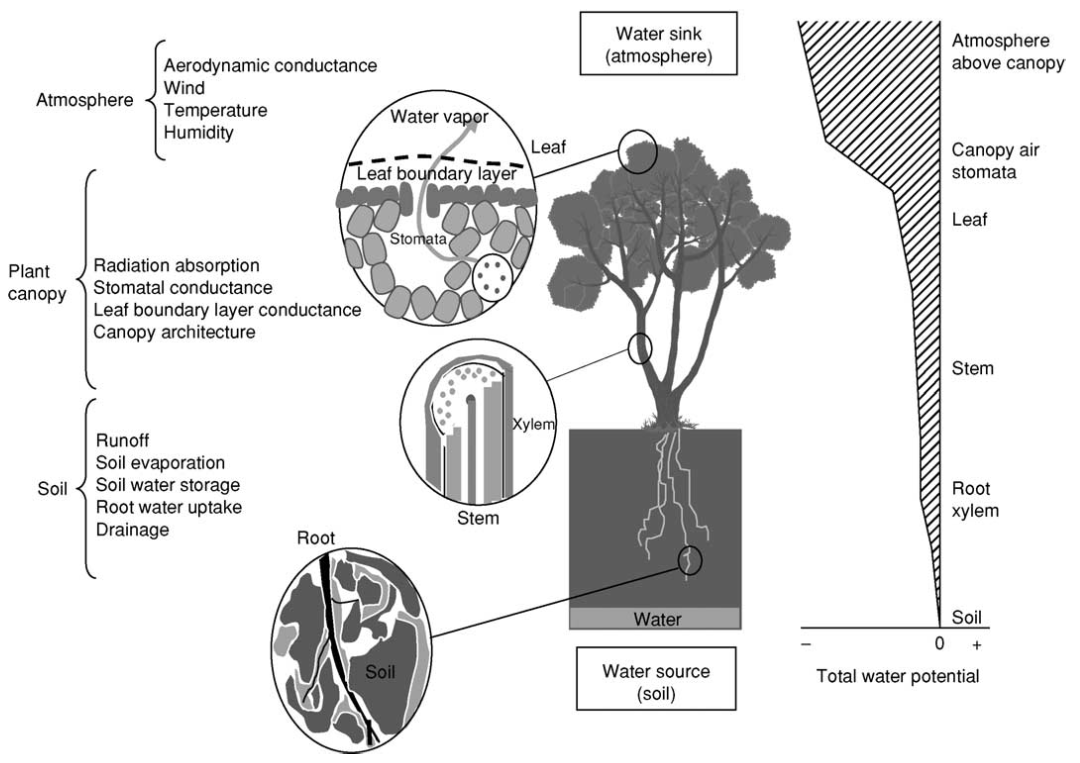
\includegraphics[width=\textwidth]{\figdir/watermovement.png}
	 	\caption{Water movement in plant due to transpiration at the leaf surface \citep{Sawinski2011}.}
	 	\label{fig:watermovement}
	 \end{figure}



\subsubsection*{Root water uptake}

An important aspect of the soil-plant-atmosphere continuum model is the root water uptake. Similar to the representing leaves in the air domain as porous media, the roots are typically represented in the soil as a sink in the water transport model. The root uptake is commonly modeled as a bulk sink term \citep{Hopmans2002,Vrugt2001}, where the net root water uptake is given as:
	 \begin{equation}
	 G_{\textit{root}} = G_{\textit{leaf}}
	 \end{equation}
	 
More recently, authors have employed a spatially varying root uptake model to study the influence of non-uniform soil moisture and dynamics such as hydraulic redistribution \citep{Volpe2013,Manoli2014a,Huang2017, Lai2000, Manoli2014}. However, the focus of these studies is on the hydrological phenomena of the soil and less on the atmospheric changes due to the plant transpiration. Therefore, there is a lack of understanding of how the water availability and the resulting dynamics have an influence on the climate above the ground. 
	
\section{Need for further research}

The present thesis aims to address the main research need as found based on the literature review. The main gap is the lack of an integrated numerical model that can simultaneously answer the following questions:
\begin{itemize}
	\item How does vegetation modify the urban heat, mass, momentum, and radiative fluxes at an urban microscale?
	\item What is the influence of environmental and plant condition on the natural cooling (transpirative and shadowing) provided by vegetation?
	\item How does the water stress affect the cooling provided by vegetation?
	\item What is the influence of vegetation on pedestrian thermal comfort?
\end{itemize}

There is a need for a rigorous approach that can predict the impact of transpiration from vegetation in an urban microclimate and directly assess the impact of vegetation on urban thermal comfort. Such a model can help study the cooling potential of vegetation and its potential mitigation factor. For this, a three-dimensional computational fluid dynamics (CFD) model of heterogeneous, porous vegetation needs to be developed, which calculates the turbulent momentum, heat, and mass exchanges of vegetation with the urban environment. Furthermore, as the important factor that drives the transpiration rate is the water availability at the root zone, a soil-plant continuum model is implemented to capture the full water transport cycle. This enables to investigate the water cycle between the atmosphere to the soil and then back to the environment via the vegetation. More importantly, the influence of water stress on the urban microclimate and its implication on thermal comfort can be addressed. Thus, the developed modeling framework aims to investigate the response of vegetation in an urban environment for various climate conditions, built and vegetation parameters.

\section{Conclusion}

The present chapter, reviewing the state of the art, provided a brief background and introduction to the urban climate discussing various urban climate scales, energy balances and the influence of vegetation at the microclimate scale. A brief study of various experimental techniques showed that wind tunnels experiments provide a level of control on the air flow condition that is not possible with field measurements. However, the cost is that smaller plants have to be used to ensure a minimal blockage effect inside the tunnel. In this thesis, wind tunnel measurements with small natural and model trees will be investigated to experimentally assess the impact of the plant on airflow and other microclimatic parameters such as air temperature and relative humidity. For an effective assessment, the experimental studies will be divided into two campaigns. The first part will investigate the impact of vegetation on the airflow. The aim will be to understand how the sheltering provided by small model trees differs from that of small natural trees and subsequently quantify the difference with mature trees. The second measurement campaign will assess the impact of vegetation on the microclimate through the use of a small \textit{Buxus sempervirens} plant. The literature review showed high-resolution measurement is possible with non-intrusive imaging techniques such as particle image velocimetry (PIV). Therefore, the flow field velocity statistics will be measured using stereoscopic particle image velocimetry (SPIV). A brief study of various numerical techniques showed that CFD methods are optimal at assessing the urban microclimate flow. Furthermore, we see that there is a need for an integrated approach that couples the conditions of the atmosphere with soil properties to determine the impact of water availability on the transpirative cooling potential of trees. So, a coupled model is to be developed to assess the hygrothermal impact of vegetation on the urban microclimate. The soil-plant-atmosphere continuum (SPAC) model will be used to link the plant transpiration with the soil moisture. The present thesis aims at assessing the impact of vegetation on the urban microclimate by understanding the influence of vegetation on turbulent urban airflow, the influence of transpiration on hygrothermal conditions, the influence of plant shading on the urban climate, and finally, the net effect on the pedestrian thermal comfort.